 \documentclass[11pt, oneside,a4paper]{book}
\pagestyle{headings}


%=============================================================================

\usepackage{amsthm}
\usepackage{xspace}
\usepackage{float}
\usepackage{ifthen}
\usepackage{amsbsy}
\usepackage{amssymb}
\usepackage{balance}
\usepackage{booktabs}
\usepackage{graphicx}
\usepackage{rotating}
\usepackage{multirow}
\usepackage{needspace}
\usepackage{microtype}
\usepackage{bold-extra}
\usepackage{geometry}
\usepackage{varioref}
\usepackage{xcolor}
\usepackage{textcomp}
\usepackage{listings}
\usepackage[normalem]{ulem} %emphasize still italic
\usepackage{ucs}

% \usepackage[utf8]{inputenc}
% \usepackage[htt]{hyphenat}
\usepackage{times}
\usepackage{url}
\usepackage{alltt}
\usepackage{amsmath}
\usepackage{xfrac}
\usepackage{subfigure}
\usepackage{appendix}
\usepackage{stmaryrd}   % for the \shortuparrow
\usepackage[utopia]{quotchap}

\usepackage{setspace}

%allow to change space between lines
\renewcommand{\baselinestretch}{1.2} 

\usepackage[numbers, sort&compress]{natbib}
\usepackage{mdwlist}        % support for better spaced lists
% allows for temporary adjustment of side margins
\usepackage{chngpage}
\usepackage[normalem]{ulem} 

\usepackage{enumitem}
\usepackage{capt-of}
% constants

\newcounter{qcounter}

% commands
\newcommand{\n}{$\cdot$}
\newcommand{\y}{\checkmark}
\newcommand{\subscript}[1]{$_{\textrm{\footnotesize{#1}}}$}
\newcommand{\superscript}[1]{$^{\textrm{\footnotesize{#1}}}$}
\newcommand{\vertical}[1]{\raisebox{-4em}{\begin{sideways}{#1}\end{sideways}}}



\newboolean{showedits}
\setboolean{showedits}{true} % toggle to show or hide edits
\ifthenelse{\boolean{showedits}}
{
       \newcommand{\ugh}[1]{\textcolor{red}{\uwave{#1}}} % please rephrase
       \newcommand{\ins}[1]{\textcolor{blue}{\uline{#1}}} % please insert
       \newcommand{\del}[1]{\textcolor{red}{\sout{#1}}} % please delete
       \newcommand{\chg}[2]{\textcolor{red}{\sout{#1}}{\ra}\textcolor{blue}{\uline{#2}}} % please change   
	\newcommand\brs[1]{\nbc{BRS}{#1}{blue}}       
       \newcommand{\nbc}[3]{
 {\colorbox{#3}{\bfseries\sffamily\scriptsize\textcolor{white}{#1}}}
 {\textcolor{#3}{\sf\small$\blacktriangleright$\textit{#2}$\blacktriangleleft$}}}
 

}{
       \newcommand{\ugh}[1]{#1} % please rephrase
       \newcommand{\ins}[1]{#1} % please insert
       \newcommand{\del}[1]{} % please delete
       \newcommand{\chg}[2]{#2}
       \newcommand{\nbc}[3]{}
}

	\newcommand\ho[1]{\nbc{H.}{#1}{violet}}
	
% ============================================================================
% Put edit comments in a really ugly standout display

\usepackage{xcolor}
\usepackage[normalem]{ulem}
\newcommand{\ra}{$\rightarrow$}


% comments \nb{label}{color}{text}
\newboolean{showcomments}
\setboolean{showcomments}{true}
\ifthenelse{\boolean{showcomments}}
    {\newcommand{\nb}[3]{
        {\colorbox{#2}{\bfseries\sffamily\scriptsize\textcolor{white}{#1}}}
        {\textcolor{#2}{\sf\small$\blacktriangleright$\textit{#3}$\blacktriangleleft$}}}
     \newcommand{\version}{\emph{\scriptsize$-$Id$-$}}
%	 \newcommand{\ugh}[1]{\textcolor{red}{\uwave{#1}}} % please rephrase
%	 \newcommand{\ins}[1]{\textcolor{blue}{\uline{#1}}} % please insert
%	 \newcommand{\del}[1]{\textcolor{red}{\sout{#1}}} % please delete
%	 \newcommand{\chg}[2]{\textcolor{red}{\sout{#1}}{\ra}\textcolor{blue}{\uline{#2}}} % please change
	 \newcommand{\chk}[1]{\textcolor{ForestGreen}{#1}} % changed, please check
	}
    {\newcommand{\nb}[3]{}
     \newcommand{\version}{}
	\newcommand{\chk}[1]{} % changed, please check
	}

% ============================================================================
% Make quotes be italic
\renewenvironment{quote}
    {\list{}{\rightmargin\leftmargin}%
     \item\relax\begin{it}}
    {\end{it}\endlist}

\newcommand{\ttimes}{\ensuremath{\times}}

%=============================================================================

\newcommand{\needlines}[1]{\Needspace{#1\baselineskip}}

% source code
\usepackage{xcolor}
\usepackage{textcomp}
\usepackage{listings}
\definecolor{source}{gray}{0.9}
\lstset{
	language={},
	% characters
	tabsize=3,
	upquote=true,
	escapechar={!},
	keepspaces=true,
	breaklines=false,
	alsoletter={:},
	breakautoindent=true,
	columns=fullflexible,
	showstringspaces=false,
	basicstyle=\footnotesize\ttfamily,
	% background
	frame=single,
    framerule=0pt,
	backgroundcolor=\color{source},
	% numbering
	numbersep=5pt,
	numberstyle=\tiny,
	numberfirstline=true,
	% captioning
	captionpos=b,
	numberbychapter=false,
	% formatting (html)
	moredelim=[is][\textbf]{<b>}{</b>},
	moredelim=[is][\textit]{<i>}{</i>},
	moredelim=[is][\uline]{<u>}{</u>}}
\newcommand{\ct}{\lstinline[backgroundcolor=\color{white},basicstyle=\footnotesize\ttfamily]}
\newcommand{\lct}[1]{{\small\tt #1}}

% end of json listing

%----------------------------------------------------------------------------
% references
\newcommand{\tabref}[1]{\hyperref[{tab:#1}]{Table~\ref*{tab:#1}}}
\newcommand{\figref}[1]{\hyperref[{fig:#1}]{Figure~\ref*{fig:#1}}}
\newcommand{\secref}[1]{\hyperref[{sec:#1}]{Section~\ref*{sec:#1}}}
\newcommand{\lstref}[1]{\hyperref[{lst:#1}]{Listing~\ref*{lst:#1}}}
\newcommand{\charef}[1]{\hyperref[{cha:#1}]{Chapter~\ref*{cha:#1}}}
%----------------------------------------------------------------------------

% abbreviations
\tracingcolors 4
\setcounter{tocdepth}{3}
\setcounter{secnumdepth}{3}
\newcommand{\ie}{\emph{i.e.,}\xspace}
\newcommand{\eg}{\emph{e.g.,}\xspace}
\newcommand{\etc}{\emph{etc.}\xspace}
\newcommand{\etal}{\emph{et al.}\xspace}


\newcommand{\newevenside}{
	\ifthenelse{\isodd{\thepage}}{\newpage}{
	\newpage
        \phantom{placeholder} % doesn't appear on page
	\thispagestyle{empty} % if want no header/footer
	\newpage
	}
}

\def\stretchfactor{1}
\newcommand{\mychapter}[1]{\setstretch{1}
    \chapter{#1}\setstretch{\stretchfactor}}

%----------------------------------------------------------------------------
\newcommand{\lessSpace}{\vspace{-1em}}
\DeclareGraphicsExtensions{.pdf,.png}
\graphicspath{{images/}}
\newcommand{\fig}[4]{
	\begin{figure}[#1]
		\centering
		\includegraphics[width=#2\textwidth]{#3}
		\lessSpace
		\caption{\label{fig:#3}#4}
	\end{figure}}

% ===========================================================================

%:CONFIGURE THIS

\newcommand{\thesistitle}{Citation Search Engine}
\newcommand{\thesisauthor}{Aliya Ibragimova}
\newcommand{\thesisauthorOrigin}{University of Fribourg}
\newcommand{\thesisleiter}{Prof.\ Dr.\ Oscar Nierstrasz}
\newcommand{\thesisasst}{Mr. Haidar Osman, Mr. Boris Spasojevic}
\newcommand{\thesisurl}{http://scg.unibe.ch/}
\newcommand{\thesissubtitle}{Academic paper search engine}
\newcommand{\thesisdate}{2015}

% ===========================================================================

\usepackage[ colorlinks=true, urlcolor=black, linkcolor=black,
			citecolor=black, bookmarksnumbered=true, bookmarks=true,
			plainpages=false,
			pdftitle={\thesistitle}, pdfauthor={\thesisauthor},
			pdfsubject={\thesissubtitle}, pdfpagelabels]{hyperref}

\newcommand{\hrref}[2]{\hyperref}
% ===========================================================================
% ===========================================================================


% D O C U M E N T
% % % % % % % % % % % % % % % % % % % % % % % % % % % % % % % % % %
\begin{document}

% T I T L E
% % % % % % % % % % % % % % % % % % % % % % % % % % % % % % % % % %
\begin{titlepage}  
  \begin{center}  
  
  \begin{figure}[t]  
  \vspace*{-2cm}        % to move header logo at the top 
  \center{
\includegraphics[scale=0.2]{logos/MSc_quer.png}}
  \vspace{0.4in}     
  \end{figure}

    \thispagestyle{empty}
    
    {\bfseries\Huge \thesistitle \par
    \Large \vspace{0.1in} \thesissubtitle \par}

    \vspace{0.3in} 
    \LARGE{\textbf{Master Thesis} \\}
    \vspace{0.4in}

    %{\Large \thesisauthor \par \thesisauthorOrigin}
    
    \vspace{0.3in}
    {\Large Faculty of Natural Sciences\\
            University of Bern \par}
    \vspace{0.3in}
    {\Large January \thesisdate \par}
    \vspace{0.3in}
    %Leiter der Arbeit: \par
   {\Large \thesisleiter} \par
      {\Large \thesisasst} \par
   \vspace{0.1in}
    {\Large Software Composition Group \par Institut f\"{u}r Informatik und angewandte Mathematik \par University of Bern, Switzerland \par}
  

  \vspace{0.9in}
 
  % === Logos ==============================================     
  \begin{figure}[htp]
    \centering
    
\includegraphics[scale=0.30]{logos/UNI_Bern.png}\hfill
    
\includegraphics[scale=0.30]{logos/UNI_Neuenburg.png}\hfill
    
\includegraphics[scale=0.80]{logos/UNI_Fribourg.png}
  \end{figure}
  % === // Logos ===========================================    


  \end{center}

\end{titlepage}


% A B S T R A C T
% % % % % % % % % % % % % % % % % % % % % % % % % % % % % % % % % %
\chapter*{\centering Abstract}
\begin{quotation}
\noindent 
Nowadays the amount of documents in World Wide Web grows exponentially. Tools that can facilitate information retrieval present a particular interest in the modern world. A typical web search engine that search
for information in World Wide Web is a software system that performs full-text indexing without considering meta information. This paper is devoted to the design of the academic paper search engine that takes advantage of meta-information, specifically citations. It is believed that citation is a very concise statement describing the source it refers to. Retrieving such statements can be particularly useful in writing scientific papers, for example, to build up a good argument.
This paper describes implementation of Citation Search Engine, a system that makes an attempt to automatically extract, index and aggregate citations from a set of scientific articles in PDF format. Besides it analyses the results of the deployment of the system on the collection of scientific papers provided by Software Composition Group.

\end{quotation}
\clearpage


% C O N T E N T S 
% % % % % % % % % % % % % % % % % % % % % % % % % % % % % % % % % % % % % % % %
\tableofcontents

%%%%%%%%%%%%%%%%%%%%%%%%%%%%%%%%%%
%%%% NEW CHAPTER %%%%%%%%%%%%%%%%%%%%%
%%%%%%%%%%%%%%%%%%%%%%%%%%%%%%%%%%
\chapter{Introduction}
\label{cha:introduction}

\section{Thesis statement}
We believe that considering meta information helps to build enhanced search systems that can facilitate information retrieval. Particularly, we target information retrieval for scientific papers. We consider citations as important text blocks summarising or judging previous scientific findings assisting in creating a new scientific work. We propose Citation Search Engine a software system that extracts citations from scientific papers, aggregates citations based on the referred source, then indexes extracted content. It provides a practical web interface that allows users to search for citations. 

\section{Goals}
We set following goals:
\begin{itemize}
	\item Introduce the state of the art techniques in information search.
	\item Explore the structure of scientific articles, reveal common patterns
	\item Design and implement the academic search engine.
	\item Deploy the system on the given collection of scientific papers
	\item Analyse results, define future work
\end{itemize}

\section{Outline}
The rest of the paper structured as follows:
\begin{description}
	\item[Chapter 2] The chapter first gives a high overview of the architecture of a typical web search engine and shortly reviews popular academic search engines. Then It describes the main steps for inverted index construction.
	%\item[Chapter 3] Devoted to the exploring the structure of scientific papers and identifying parsing challenges.
	\item[Chapter 3] Describes the design of Citation Search Engine. It first shows overall architecture of the proposed system and then describes details of implementation of each component. 
	\item[Chapter 4] The chapter describes the deployment process and analysis the result of setting up the system on the given collection of scientific articles.
	\item[Chapter 5] Evaluation
	\item[Chapter 6] Contains conclusion and possible future work. 
\end{description}

\chapter {Related Work}
\section{Typical web search engine} 

Figure \ref{fig:web-search} illustrates a high level architecture of a standard web engine. It consist of three main components:
\begin{itemize}
	\item Web Crawler
	\item Data indexer
	\item Search interface
\end{itemize} 

  \begin{figure}[htp]
    \centering
    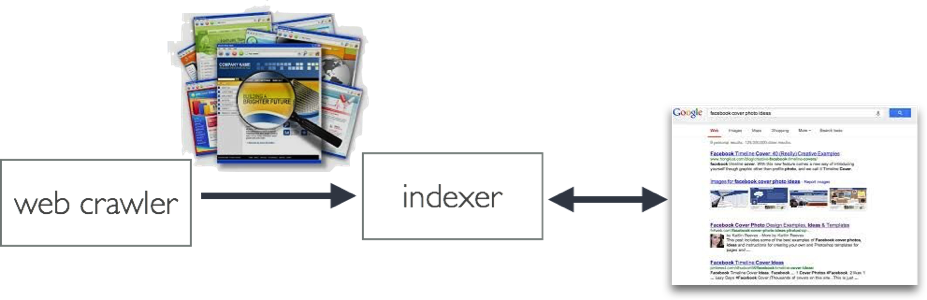
\includegraphics{web-search-engine}
    \caption{A high-level architecture of a typical web search engine}
    \label{fig:web-search}
  \end{figure}

Web Crawler is a program that browses the World Wide Web reading the content of web pages in order to provide up-to-date data to Data Indexer. Data Indexer decides how a page content should be stored in an index database. Index helps to quickly query information. Users can search and view query results through Search Interface. When user makes a query the search engine analysis its index and returns best matched web pages according to specific to indexer criteria. 

Web crawlers that fetch web pages with the content in the same domain are called focused or topical crawlers. An example of focused crawlers are academic-focused crawlers that crawls academical documents. Such crawlers become components of the "focused" search engines. Next chapter reviews some of popular academical search engines.  

\section{Popular academic search engines}
\paragraph{CiteSeer\textsuperscript{x}}
CiteSeer\textsuperscript{x} is an autonomous citation search engine \cite{citeseer, Giles:1998:CAC:276675.276685}. CiteSeer\textsuperscript{x} automatically parses and index publicly available scientific articles found on the World Wide Web. It uses the impact of citations to rank documents.
CiteSeer\textsuperscript{x} is built on the open source infrastructure SeerSuite \cite{seersuite} and uses Apache Solr \cite{solr} search platform for indexing documents. It can extract meta information from papers such as title, authors, abstract, citations. The extraction methods are based on machine learning approaches such ParseCit \cite{Councill08parscit:an}. 
CiteSeer\textsuperscript{x}  one of the world's top repositories and was rated number 1 in July 2010 \cite{web-repos}. It currently has over 4 million documents with nearly 4 million unique authors and 80 million citations. 
CiteSeer\textsuperscript{x} focuses on indexing citations more precisely bibliographic links while in Citation Search Engine we intend to index text of the citations in a body of a document.
\\ \\
\textbf{Google Scholar} 
Google Scholar is a freely accessible web search engine that makes full-text indexing of scientific literature \cite{google.scholar}. Among features of Google Scholar engine are unique ranking algorithm, "cited by" feature, allowing to view abstracts of the articles citied the given article, "related articles" feature, showing the list of closely related articles.
Google Scholar contains roughly 160 million of documents by May 2014 \cite{orduna2014size}. 

\section{Inverted index}
Search engines like CiteSeer or Google Scholar deal with a large collection of documents. When user makes a query to such systems one would like to have a mechanism to process document collections quickly. The way to avoid linear scanning the text of all documents for each query is to \emph{index} them in advance. Thereby we are coming to the concept of \emph{inverted index} that is the major concept in information retrieval. The term \emph{inverted index} comes from the data structure storing a mapping from content, such as words or numbers, to the parts of a document where it occurs. Figure \ref{fig:inverted-index} shows the basic idea of an inverted index. We have a dictionary of terms appearing in the documents. Each term maps to a list that records which documents the term occurs in. Each item in the list, conventionally named as \emph{posting}, records that a term appears in a document, often it records the position of the term in the document as well. The dictionary on Figure \ref{fig:inverted-index} has been sorted alphabetically and each postings list is sorted by document ID. Document ID is a unique number that can be assigned to a document when it's first encountered. \\
  \begin{figure}[htp]
    \centering
    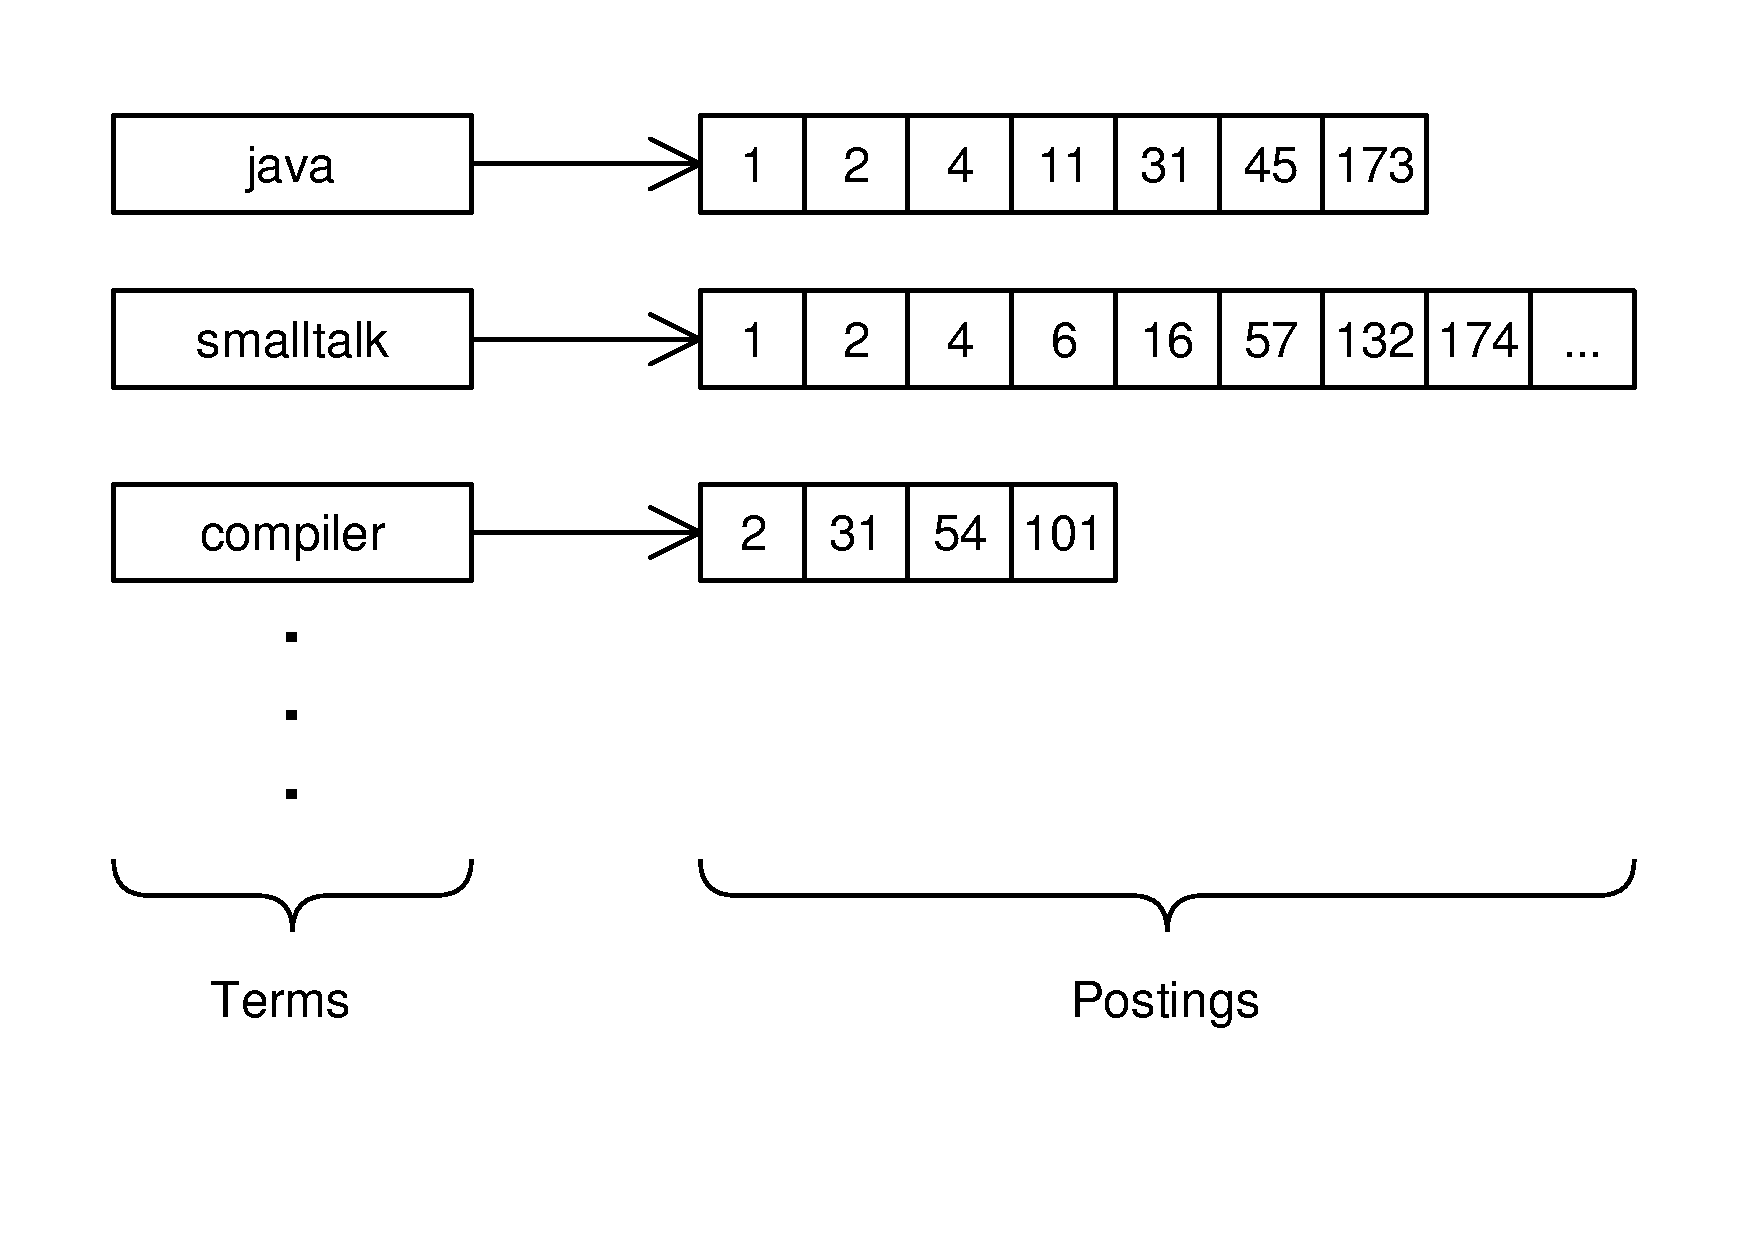
\includegraphics[scale=0.55]{inverted-index}
    \caption{Inverted index example}
    \label{fig:inverted-index}
  \end{figure}
  
 The construction of the inverted index has following steps:
 
\begin{enumerate}
	\item Documents collection
	\item Breaking each document into tokens, turning a document into a list of tokens
  	\item Linguistic preprocessing of a list of tokens into normalised list of tokens
	\item Index documents by creating  an inverted index, consisting of a dictionary and postings
\end{enumerate}

First step of the index construction is documents collection that aims to obtain a set of documents containing sequence of characters. Usually the input to the indexing process is digital documents that are bytes in a file or a web server. While for the plain English text in ASCII encoding solution is straightforward there might be trickier cases. Consider for example a collection of PDF files, we need to correctly decode out characters of some binary representation. Finally, the textual part of the document may need to be extracted out of other parts that will not be processed. Next we should determine a document unit, for example it might be a chapter in a book, or a paragraph in a scientific article. 

After getting the sequence of characters in document units next step is to breaking up documents into \emph{tokens}. Token can be think of a semantical unit for processing, for example, it might be a word or a number. At the same time during tokenisation some characters like punctuations can be thrown out. 

Here is a tokenisation example:

\hspace{50pt}\textcolor[rgb]{0,0,1}{ Input: Friends, Romans, Countrymen, lend me your ears; }

\hspace{50pt}\textcolor[rgb]{0,0,1}{Output: \framebox{Friends} \framebox{Romans} \framebox{Countrymen} \framebox{lend} \framebox{me} \framebox{your} \framebox{ears}} \\

The third step is normalization. It's good when tokens in a user query match tokens in the token list of documents. Consider an example of querying the word \emph{co-operation}, a user might also be interested in getting documents containing \emph{cooperaion}. \emph{Token normalisation} is a process of turning a token into a canonical form so matches can occur despite superficial differences in the character sequences. One way of token normalisation is keeping relations between unnormalized tokens, which can be extended to manual constructed synonym lists, such as \emph{car} and \emph{automobile}. The most standard way of token normalization however is creating \emph{equivalence classes}. If tokens become identical after applying a set of rules then they are the equivalence classes. Consider some common normalization rules that are often used:

\begin{description}
	\item[Stemming and lemmatization] Words can be used in different grammatical forms, for instance, \emph{organize}, \emph{organizes}, \emph{organizing}, however in many cases it sounds reasonable for one of these words to return documents contain other forms of the word. The goal of stemming and lemmatization is reduce a form of the word to a common base form. 
	
Here is an example: 
	
\hspace{100pt} \textcolor[rgb]{0,0,1}{ am, are, is = \textgreater be }

\hspace{100pt} \textcolor[rgb]{0,0,1}{car, cars, car's, cars'  =\textgreater car}

The result of applying the rule to the sentence:

\hspace{50pt} \textcolor[rgb]{0,0,1}{the boys cars are different colors   =\textgreater the boy car be differ color}

Stemming and lemmatization are closely related concepts however there is a difference. \emph{Lemmatization} usually refers to finding a \emph{lemma}, common base of a word, with the help of a vocabulary, morphological analysis of a word and requires understanding the context of a word and language grammar. \emph{Stemming} however operates with a word without knowing it context and thereby can't distinguish the same words having different meanings depending on the context. 

Here is an example:

\hspace{10pt} \textcolor[rgb]{0,0,1}{ better = \textgreater good }, can only be matched by lemmatization since requires dictionary look-up

\hspace{10pt} \textcolor[rgb]{0,0,1}{writing  =\textgreater write}, can be matched by both lemmatization and stemming

\hspace{10pt} \textcolor[rgb]{0,0,1}{meeting  =\textgreater meeting(noun) or to meet(verb)}, can be matched only by lemmatization since requires the word context 

In general stemmers are easier to implement and run faster. The most common algorithm for stemming is \emph{Porter's} algorithm \cite{Porter:1997:ASS:275537.275705}.
	  
	\item[Capitalization/case-folding] A simple strategy is to reduce all letters to a lower case, so that sentences with \emph{Automobile} will match to queries with \emph{automobile}., however this approach would not be appropriate for example to identifying company names, such as \emph{General Motors}. The better strategy for English language would be to lowercase words only in the beginning of the sentences and to lowercase all words in titles. Case-folding can be be done more accurately by a machine learning model using more features to identify weather a words should be lowercased.
	\item[Accents and diacritics]  Diacritics in English language play an insignificant role and simply can be removed. For instance \emph{clich\'e} can be substituted by \emph{cliche}. In other languages diacritics can be part of the writing system and distinguish different sounds.  However in many cases users can enter queries for words without diacritics, whether for reasons of speed, laziness or limited software 
\end{description}

The last step is the core part of the building inverted index. The input to indexing is a list of normalized tokens for each document, which is a list of pairs of
term and document ID, as on Figure \ref{fig:input-indexing}. The indexing algorithm is sorting the input list so that the terms are in alphabetical order. Then it merges the same terms from the same document. And finally instances of the same term are grouped and the result is split into a dictionary and postings, as shown on Figure \ref{fig:inverted-index}.

  \begin{figure}[htp]
    \centering
    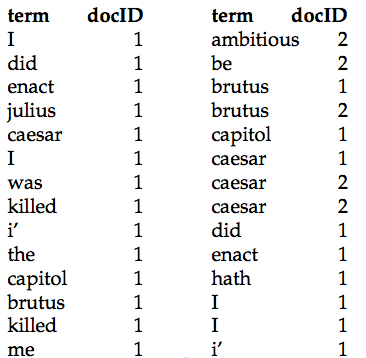
\includegraphics[scale=0.5]{input-indexing}
    \caption{Input to the indexing algorithm}
    \label{fig:input-indexing}
  \end{figure}

%%Since a term generally occurs in a number of documents, this data organization already reduces the storage requirements of the index. 

\section{Dynamic indexing}
So far we assumed that document collection is static however there are many cases when collection can be updated, for example, by adding new documents, deleting or updating existing documents. One simple way dealing with dynamic collection is to reconstruct the inverted index from scratch. This might be acceptable if changes made in collection are small over time and delay in making new documents searchable is not critical. However if there is one of a requirement mentioned above, for example, making new documents searchable quickly then one might be interested in another solution: keeping auxiliary index. Thus we have a large main index and we keep auxiliary index for changes. The auxiliary index is kept in memory. Every time a user makes a query the search runs over both of the indexes and results are merged. When auxiliary index becomes too large it can be merged with the main index.

\section{Retrieving search results}
When a user makes a query she would be interested in getting a result document containing all terms in the query so that terms are close to each other. Consider an example of querying a phrase containing 4 terms. The part of the document that contains all terms is named a \emph{window}. The size of the window is measured in a number of words. For instance a smallest  window for 4-terms query will be 4. Intuitively, smaller windows represent better results for users. Such window can become one of the indicators scoring a document in the search result. If there is no document containing all 4 terms, a 3-term phrase can be queried. Usually search systems hides the complexity of searching a result from user introducing \emph{free text query parsers} so a user can make only one query.     

\section{Search Engine - entire picture} 
Figure \ref{fig:search-full-diagram} summarizes approaches described above in a more detailed picture of a basic search system. 
Left stream in the Figure \ref{fig:search-full-diagram} describes the process of parsing a set of documents and applying linguistic processings (tokenization and lemmatization) in order to built indexes with the help of a indexer. The middle stream on Figure \ref{fig:search-full-diagram} represents a user making a query, where free text parsers together with spell checkers send requests to the index bank. The index bank returns document candidates to a scoring and ranking component, the left stream on Figure \ref{fig:search-full-diagram}. Finally, ranked document are shown to the user as a result page.    

  \begin{figure}[htp]
    \centering
    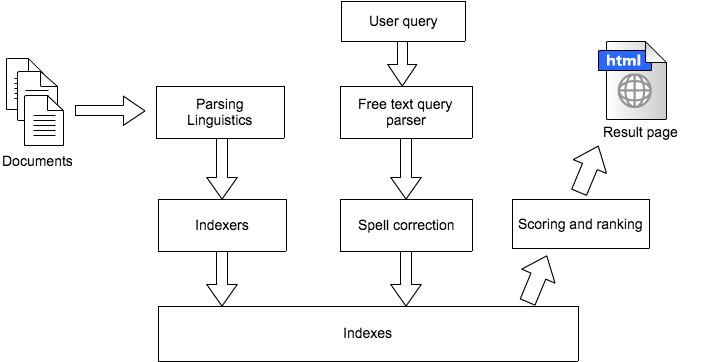
\includegraphics[scale=0.6]{search-full-diagram}
    \caption{Search Engine internals}
    \label{fig:search-full-diagram}
  \end{figure}

\section{Citations in scientific publications}
Citations remain interesting basic units for analysis in many scientific studies. 
Bradshaw et al. \cite{bradshaw} showed that citations provide many different perspectives on the same article, in their work authors improves search engine results with a method called Reference Directed Indexing. Bertin and Atanassova \cite{marc1}, \cite{M_automaticannotation} made an attempt to automatically extract citations and annotate them using set of semantic categories. There are several studies that used citations to evaluate science by introducing map of science, which graphically reflects the structure, evolution and main contributors of a given scientific field \cite{map1}, \cite{Klavans:2009:TCM:1527090.1527095}, \cite{DBLP:journals/corr/abs-1202-1914}, \cite{Small:1999:VSC:308915.308932}. An interesting approach is to use citations to build summaries of scientific publications. There are three categories of summaries proposed based on citations: overview of a research area (multi-document summarization) \cite{Nanba:1999:TMS:1624312.1624351}, impact summary (single document summary with citations from the scientific article itself) \cite{mei-zhai:2008:ACLMain} and citation summary (multi- and single document summarization, in which citations from other papers are considered) \cite{Qazvinian:2008:SPS:1599081.1599168}. In work by Nakov et al. citations have been used to support automatic paraphrasing \cite{Nakov04citances:citation}. An expert literature survey on citation analysis was made by Smith \cite{smith}, she reviewed hundred of scientific articles on this topic.      
 

%\chapter {Related Work}

%In which we understand what the problem is in detail.

\chapter {Citation Search Engine}

\section{System overview}

The overall architecture of Citation Search Engine is shown on Figure \ref{fig:cs}. There are three main operations performed by Citation Search Engine: parsing PDF files, indexing documents and querying on resulted indexes. Correspondingly there are three major components responsible for accomplishment of these operations: \emph{Parser}, \emph{Indexer Solution} and \emph{Search Web App}. The system has two more components for storing data: \emph{Indexes Storage} for storing indexes and \emph{Meta Information Storage} for storing meta information. For the convenience, the workflow of the system is numbered and will be explained below.

  \begin{figure}[htp]
    \centering
    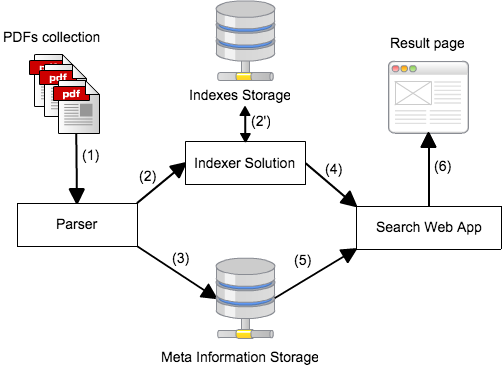
\includegraphics[scale=0.6]{cs}
    \caption{Search Engine high level architecture}
    \label{fig:cs}
  \end{figure}

First operation performed by the system is indexing. In the indexing process collection of PDF files is provided to \emph{Parser} (1). \emph{Parser} parses PDF files into text and extract meta information from text. It then packs data about citations into documents and publishes obtained documents to \emph{Indexer Solution} (2) which indexes and stores indexes in \emph{Indexes Storage} (2'). Meta information extracted from textual representation of PDF files that doesn't require indexing is stored in \emph{Meta Information Storage} (3). 

In the querying process user searches for some phrase using \emph{Search Web App} user interface. The phrase is analyzed by \emph{Indexer Solution}. \emph{Indexer Solution} finds documents matching the query phrase in \emph{Indexes Storage} (2') and sends them to \emph{Search Web App} (4). If user is interested in getting details regarding the specific reference the information will be looked up in \emph{Meta Information Storage} (5). Finally, the result is shown to the user as a an html page (6). 

Next sections of the chapter describe implementation of each component in detail and show the reasons of choosing a particular solution.       

\section{Parser}

It is practical to divide the work of \emph{Parser} into two phases: \emph{Processing} and \emph{Publishing}, as on Figure \ref{fig:parser}. The output of \emph{Processing} phase is input to \emph{Publishing} phase. \emph{Processing} phase aims to parse PDF-files and prepare documents with extracted information for publishing. Next parts of this section describes \emph{Processing} and \emph{Publishing} phases in detail. 

  \begin{figure}[htp]
    \centering
    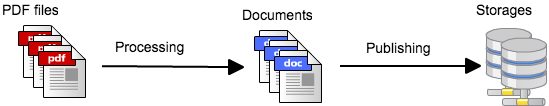
\includegraphics[scale=0.6]{parser}
    \caption{Parser workflow}
    \label{fig:parser}
  \end{figure}

\subsection{Processing}
The main role of \emph{Processing} phase is to parse scientific articles into text and extract citations and bibliographic references to create documents for publishing. 
In common case parsing PDF-files from different sources is a very challenging task as there is a large number of scientific articles in different formats. Besides that there exist scientific articles written decades ago which can use different encoding algorithms than articles created recently. Thereby building a universal parser is practically impossible. In our case we try to identify common patterns covering majority of scientific article formats or at least formats found in our collection of articles.  

\emph{Processing} phase starts with recursively walking though directory tree of the collection library. While walking though directory \emph{Parser} filters non-pdf files and parses and processes each PDF-file separately. We used Apache PDFBox library \cite{pdfbox} to parse PDF-files into text. The library extracts full text from PDF-file but without any hints on the initial structure of the article. In our case to find citations and bibliographic references in text we need to look them up in different parts of the article, so it was designed an algorithm to break PDF-text into sections.

Generally we are interested in identifying a body of the document where we can find citations and references block where we can find bibliographic links. One way of finding these sections can be using keywords that might signify the beginning or the end of some section. Based on keywords on can extract different sections of a document. Figure \ref{fig:template} shows a sample text of a parsed pdf-document with keywords. 
  
One can notice following characteristics of scientific articles:
\begin{itemize}
	\item Body of a document comes before references section
	\item Appendix or Author's biography sections can come after references section 
	\item Each document contains an Abstract and References words and might contain Appendix word. We call these words keywords. 
\end{itemize}  

In common case keywords can be written in different formats, for example, using upper or lower case. Table \ref{tab:keywords} illustrates variations of keywords in the beginning of document sections.

\begin{table}[ht]
\begin{center}
\begin{tabular}{ | l | l | l | } 
 \hline
 body & references & appendix \\  \hline
 Abstract & References & Appendix \\ 
 ABSTRACT & References: & APPENDIX \\
 & REFERENCES & \\  
 \hline
\end{tabular}
\caption{Keywords identifying different sections in a document}
\label{tab:keywords}
\end{center}
\end{table}

After breaking down a document into sections as show on Figure \ref{fig:template}, text in sections are presented in one-column format. There are two aspects regarding this format. First, sentences can be splitted by new line symbol in the end of a line. Secondly, words can be splitted by dash symbol in the end of a line. It was introduce a normalization step where new lines are substituted by white spaces and dashes are removed in the end of a line to obtain continues text.

  \begin{figure}[htp]
    \centering
    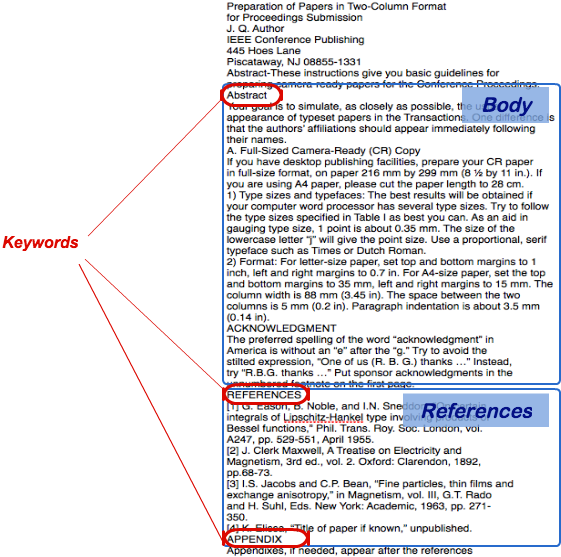
\includegraphics[scale=0.6]{template}
    \caption{Sample text of the parsed scientific article. Keywords help to break the document into sections.}
    \label{fig:template}
  \end{figure}

As a result of normalization step we have a document divided into body and references section. Before searching citations in the body of a document it is reasonable to break body into sentences. In general, breaking text into sentences is not an easy task. Consider a simple example with a period. Period not only indicates the end of a sentence but also can encounter in a sentence itself, for example, an item of a numbered list or a name of a scientist. Besides, not all sentences end by period, for example, title of a section or an item of a list. It was used Stanford CoreNLP library that employs natural language and machine learning techniques to extract sentences \cite{stanford.nlp}. 

Next, we search for citations in a body of a document and bibliography links in a references section. When an author makes a citation it puts a link to a bibliographic reference in the sentence. It is common to use square brackets ([ and ]) to make a link to a bibliographic reference in the sentence. Thus, detecting square brackets in the text we can identify citations. After analyzing some set of articles it was revealed frequent patterns in using square brackets for citing showed in Table \ref{tab:citations}. 

\begin{table}[ht]
\begin{center}
\begin{tabular}{ | l | p{7cm} | } 
 \hline
 Patterns of using [ ] & Example in text \\  \hline
 {[}21{]} & Our conclusion is that, contrary to prior pessimism \textbf{[21]}, [22], data mining static code attributes to learn defect predictors is useful. \\ 
 {[}20, 3, 11, 17{]} & In the nineties, researchers focused on specialized multivariate models, i.e., models based on sets of metrics selected for specific application areas and particular development environments \textbf{[20, 3, 11, 17]}. \\
 {[}24, Sections 6.3 and 6.4 {]}& Details on the life-cycle of a bug can be found in the BUGZILLA documentation \textbf{[24, Sections 6.3 and 6.4]}. \\
 {[}PJe02{]} & In a lazy language like Haskell \textbf{[PJe02]} this is not an issue - which is one key reason Haskell is very good at defining domain specific languages.  \\
 \hline
\end{tabular}
\caption{Frequent patterns in using square brackets ([ and ])for citing}
\label{tab:citations}
\end{center}
\end{table}


Further we need to extract bibliographic links from a references section. For that we studied most common variants of composing references sections. Table \ref{tab:references} surmises these findings. To extract bibliographic links we make list of regular expressions matching one of those patterns listing in Table \ref{tab:references}. Extracting bibliographic links allow us to match citations with bibliographic links.

\begin{table}[h]
\begin{center}
\begin{tabular}{ | p{12cm} | } 
 \hline
 References section templates\\  \hline
 \textbf{[1]} J. Bach. Useful features of a test automation system (partiii) \ldots \newline
 \textbf{[2]} B. Beizer. Black-Box Testing. John Wiley and Sons, \ldots \newline
 \ldots \\ \hline 
 \textbf{1.}  J. R. Hobbs,  Granularity, Ninth International Joint Conference \ldots \newline
  \textbf{2.}  W. Woods, What's in a Link:  Foundations for Semantic Networks, \ldots \newline
  \ldots \\ \hline
  \textbf{[1].}   Arnold, R.S., Software Reengineering, ed. \ldots \newline
  \textbf{[2].}   Larman, C., Applying  UML and Patterns. 1998, \ldots \newline  
  \ldots \\ \hline
  \textbf{[ASU86]} A. V. Aho, R. Sethi, and J. D. Ullman. Compilers: \ldots \newline
  \textbf{[AU73]} A.V. Aho and J.D. Ullman. The theory of parsing, translation \ldots \newline 
  \ldots \\
 \hline
\end{tabular}
\caption{Frequent patterns of writing references block}
\label{tab:references}
\end{center}
\end{table}

The pipeline of processing stage described above depicted on Figure \ref{fig:proc}. As seen from Figure \ref{fig:proc} to complete the processing stage we need to perform one more step: extracting titles from bibliographic links. The objective point of extracting titles from bibliographic links is to collect citations referred to the the same source (scientific article). In general case, different formats of bibliographic links can identify the same source or scientific article. For example, an article may have different editions, published in different journals in different years or simply different authors may use different style formatting. What we consider to be identical for all bibliographic links citing the same paper is the paper's title.   

  \begin{figure}[htp]
    \centering
    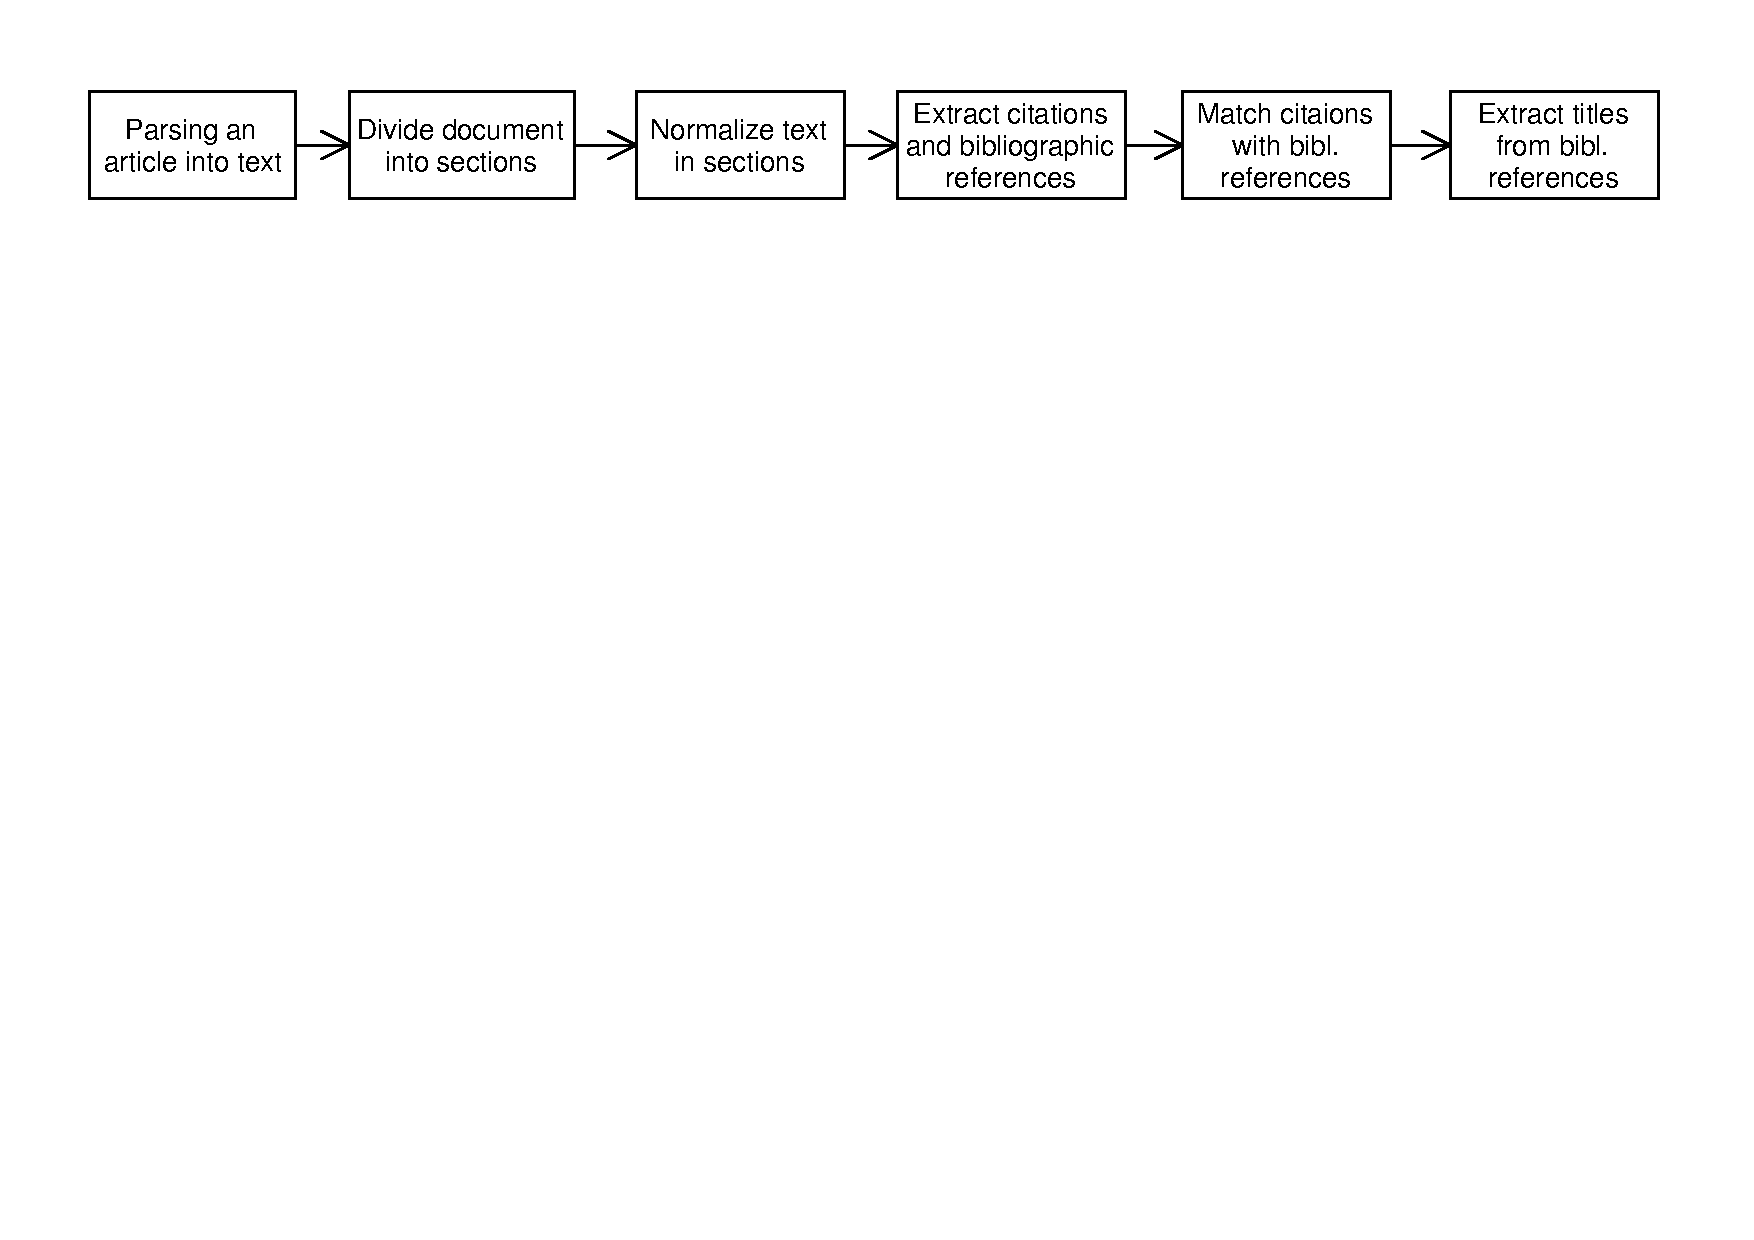
\includegraphics[scale=0.55]{processing}
    \caption{Pipeline of processing stage}
    \label{fig:proc}
  \end{figure} 

\paragraph{Processing bibliographic links}
As usual we try to recognize common patterns belonging to majority of bibliographic links. Table \ref{tab:bibl.links} shows some examples of bibliographic links. First, it was noticed that if bibliographic link contains some sort of quotes, for example, double quotes ``'' or single quotes `', then highly probably that a title is enclosed by these quotes. Then, some observations were made for bibliographic links without quotes. Very often, a bibliographic link structured as follows: it begins by listing paper's authors, then paper's title goes and then comes the rest of the link (see Figure \ref{fig:link}). It turned out that Core NLP library used for breaking text into sentences is good in dividing a link into parts according to our view. In most of cases it's enough to take the second part of the bibliographic link to be a title.   

\begin{table}[h]
\begin{center}
\begin{tabular}{ | p{12cm} | } 
 \hline
 Conradi, R., Dyba, T., Sjoberg, D.I.K., and Ulsund, T., "Lessons learned and recommendations from two large norwegian SPI programmes." Lecture notes in computer science, 2003, pp. 32-45."
 \\ \hline 
 P. Molin, L. Ohlsson, `Points \& Deviations - A pattern language for fire alarm systems,' to be published in Pattern Languages of Program Design 3, Addison-Wesley.
 \\ \hline
  R. P. Wilson and M. S. Lam. Effective context sensitive pointer analysis for C programs. In PLDI, pages 1–12, June 1995. 289 
  \\ \hline
  Allen, Thomas B. Vanishing Wildlife of North America. Washington, D.C.: National Geographic Society, 1974.
  \\ \hline
  I. Herraiz, J. M. Gonzalez-Barahona, and G. Robles. Towards a Theoretical Model for Software Growth. In Proceedings of the 4th International Workshop on Mining Software Repositories, Minnesotta, USA, May 2007.
  \\
 \hline
\end{tabular}
\caption{Some examples of bibliographic links}
\label{tab:bibl.links}
\end{center}
\end{table}

  \begin{figure}[htp]
    \centering
    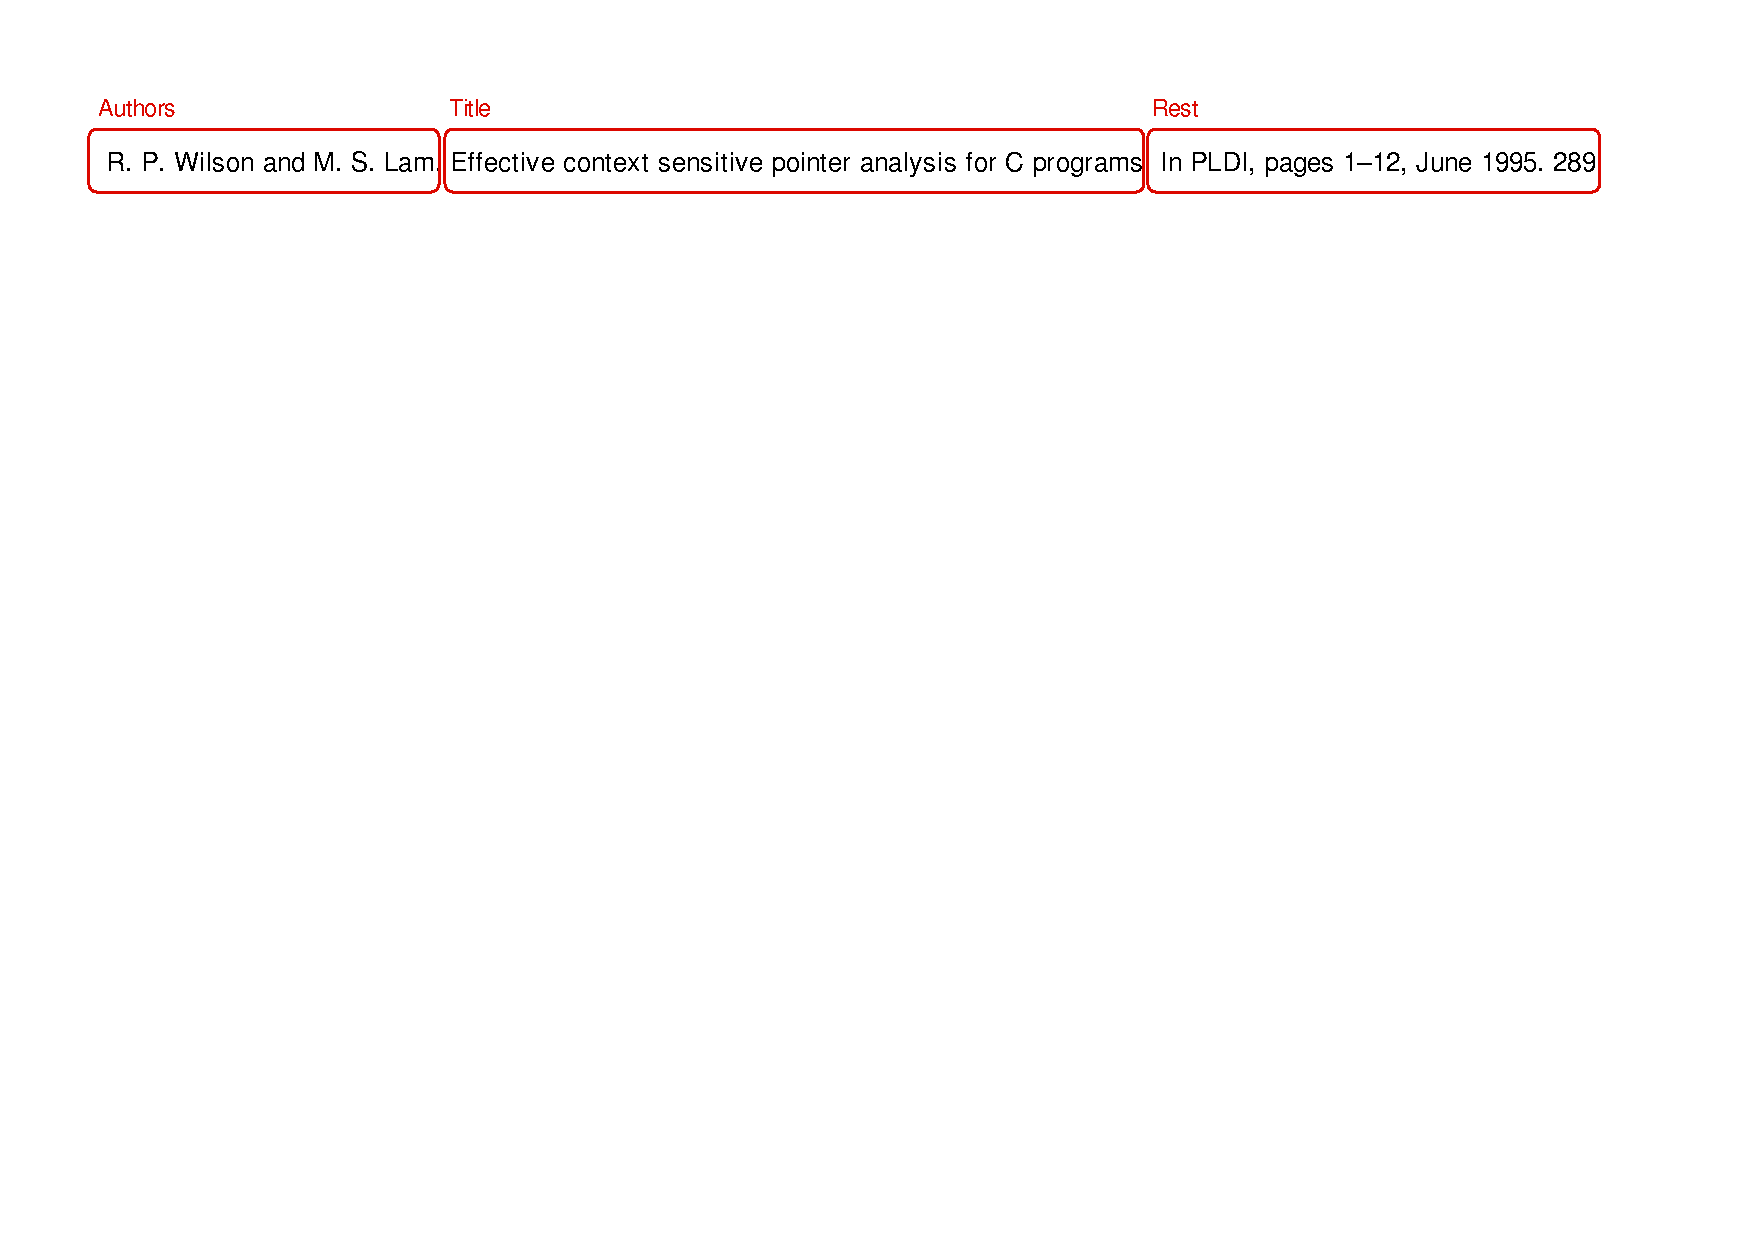
\includegraphics[scale=0.5]{link}
    \caption{Structure of a bibliographic link}
    \label{fig:link}
  \end{figure}     

\subsection{Publishing}

There are two systems where documents will be published: Solr and MongoDB. As already explained above Solr is used for indexing citations and MongoDB for storing meta-data. Some reasonings in favor of using MongoDB additionally to Solr storage will be given below.

\paragraph{Publishing to Solr}
The common way to interact with Solr is using REST API. Solr provides client libraries for many programming languages to handle interactions with Solr's REST API. In our project we used SolrJ client library for Java language. This library abstract interaction with Solr into java objects instead of using typical XML request/response format. Basic Solr storage unit is called document and SolrJ has document abstraction implementation. For every detected citation we compose a document to publish. Figure \ref{fig:doc} represents a structure of documents we publish to Solr.

  \begin{figure}[htp]
    \centering
    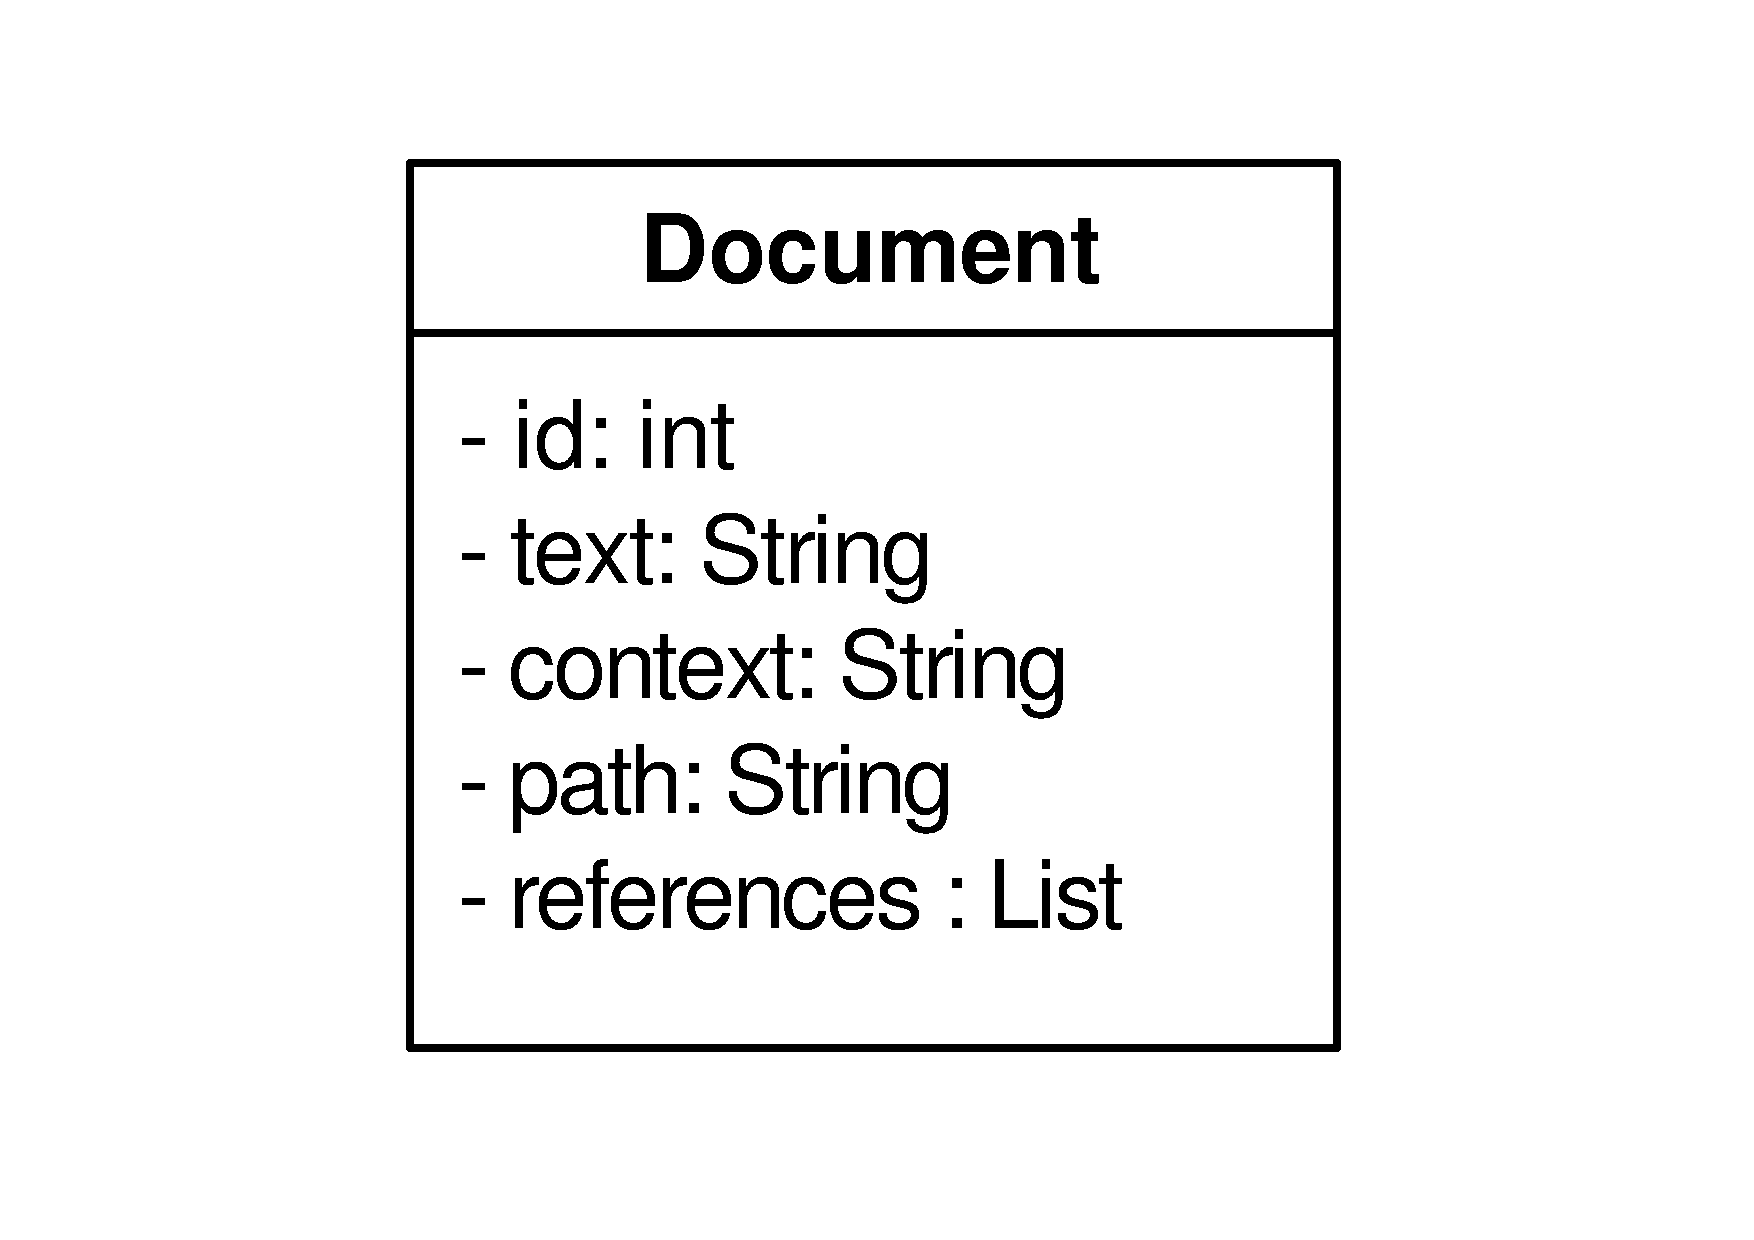
\includegraphics[scale=0.7]{doc}
    \caption{Document structure publishing to Solr}
    \label{fig:doc}
  \end{figure} 

Every document representing one citation consist of following fields:
\begin{itemize}[noitemsep]
  \item id: document unique id, mandatory field for publishing to Solr
  \item text: text of the citation that we want to index
  \item context: citation with a text framing it, we take 1 sentence before and 1 after the citation 
  \item path: URL of a document where citation was found
  \item references: list of bibliographic links from references section matching this citation
\end{itemize}

Lets have a look at how Solr stores documents. Solr uses NoSQL like data storage, but actually it is even more limited than traditional NoSQL databases. Indeed, the data stored in Solr storage is very `flat', which means that Solr doesn't allow to store even hierarchical data \cite{use.solr1}, \cite{use.solr.2}. In our case along with the references we intent to store a title of the scientific article parsed from the reference string, so later we can aggregate citations referred to the same scientific article. /*It's worth to say that citation itself can refer to multiple scientific articles*/ We are also interested in a solution that doesn't require reviewing all Solr documents to find citations referred to the same scientific article as it will be too slow and will decrease quality of user experience. Thus we are coming to the external storage solution that will keep titles of scientific articles and all citations referred to a specific article. As there are few relations in our data and we would like to have a scalable solution it was decided to use MongoDB as an external storage.     

\paragraph{Publishing to MongoDB} 
MongoDB is a document-oriented NoSQL database that stores data in JSON-like documents with dynamic schema \cite{mongo}. To connect to database we used Java driver provided by MongoDB. Although MongoDB is a `schemaless' database we adhere to JSON structure of a document showed on Listing \ref{lst:json}. 
The json document consist of following fields:
\begin{itemize}[noitemsep]
	\item id: document id, field automatically assigned by MongoDB
	\item title: title of a scientific article
	\item cittations: citations with its references of the scientific article identifying by title field 
\end{itemize} 

Every time while sending a new citation with paper title to MongoDB we check if document with the same title already exist. If so we add a new citaion to this document otherwise create a new document. \\

\begin{minipage}{\linewidth}
\begin{lstlisting}[label={lst:json}, caption={Sample document stored in MongoDB}]
{ 
	"_id" : ObjectId("547ef1b219795f049d6a0ad0"), 
	"title" : "Re-examining the Fault Density-Component Size  Connection", 
	"citations" : [ 
	{ 
		"citation" : "Hatton, [19], claims that there is “compelling empirical 
					  evidence from disparate sources to suggest that in any 
					  software system, larger components are proportionally more 
					  reliable than smaller components.”", 
		"references" : [ 
		"[19] L. Hatton, “Re-examining the Fault Density-Component Size ..." 
		] 
	}, 
	{ 
		"citation" : "Hatton examined a number of data sets, [15], [18] and 
					  concluded that  there was evidence of “macroscopic behavior” 
					  common to  all data sets despite the massive internal 
					  complexity of each  system studied, [19].", 
		"references" : [ 
		"[15] K.H. Moeller and D. Paulish, “An Empirical Investigation of ...", 
		"[18] T. Keller, “Measurements Role in Providing Error-Free Onboard ...", 
		"[19] L. Hatton, “Re-examining the Fault Density-Component Size  ..." 
		] 
	}] 
}
\end{lstlisting}
\end{minipage}

\subsection{Challenges}

%We want to establish the link between sentences containing citations (and therefore reference keys) in the text and the corresponding bibliographic references in the bibliography of the publication. This task is straightforward if the reference keys are in numerical or alphanumerical form (e.g. '[75]', '[BER08]') because in this case they are also present at the beginning of the corresponding reference in the bibliography. The difficulty arises when the bibliography style does not include the reference keys themselves and the keys present in the text are formed from the authors' names and the year using a specific syntax that may vary from one publication to another. This type of reference keys is more often used in human and social sciences. A classification of the different types of reference keys in scientific texts has been proposed by 

\section{Indexator}

As an Indexator we use Solr: solution from Apache Software Foundation built on Apache Lucene. Apache Lucene is an open source, information retrieval library that provides indexing and full text search capabilities \cite{lucene}. While web search engines focus on searching content on the Web, Solr is designed to search content on corporate networks of any form. Some of the public service that use Solr as a server: Instagram (photo and video sharing social network), Netflix (movie hosting service), StubHub.com (public entertainment events ticket reseller). 

Figure \ref{fig:solr} illustrates a high level architecture of Solr. Solr is distributed as a Java web application that runs in any servlet container, for example, Tomcat or Jetty. It provides REST-like web services so external applications can make queries to Solr or index documents. Once the data is uploaded, it goes through text analysis pipeline. In this stage, different inspections to remove duplicates in the data or some document-level operations prior to indexing, or create multiple documents from a single one can be applied. Solr comes with variety of query parser implementations responsible for parsing the queries passed by the end search as a search string. For example, \emph{TermQuery, BooleanQuery, PhraseQuery, PrefixQuery, RangeQuery, MultiTermQuery, FilteredQuery, SpanQuery} and others. Solr has xml configuration files (schema.xml and solrconfig.xml) to define the structure of the index and how fields will be represented and analyzed.

Next section describes configuration of Solr instance for our search system.  

  \begin{figure}[htp]
    \centering
    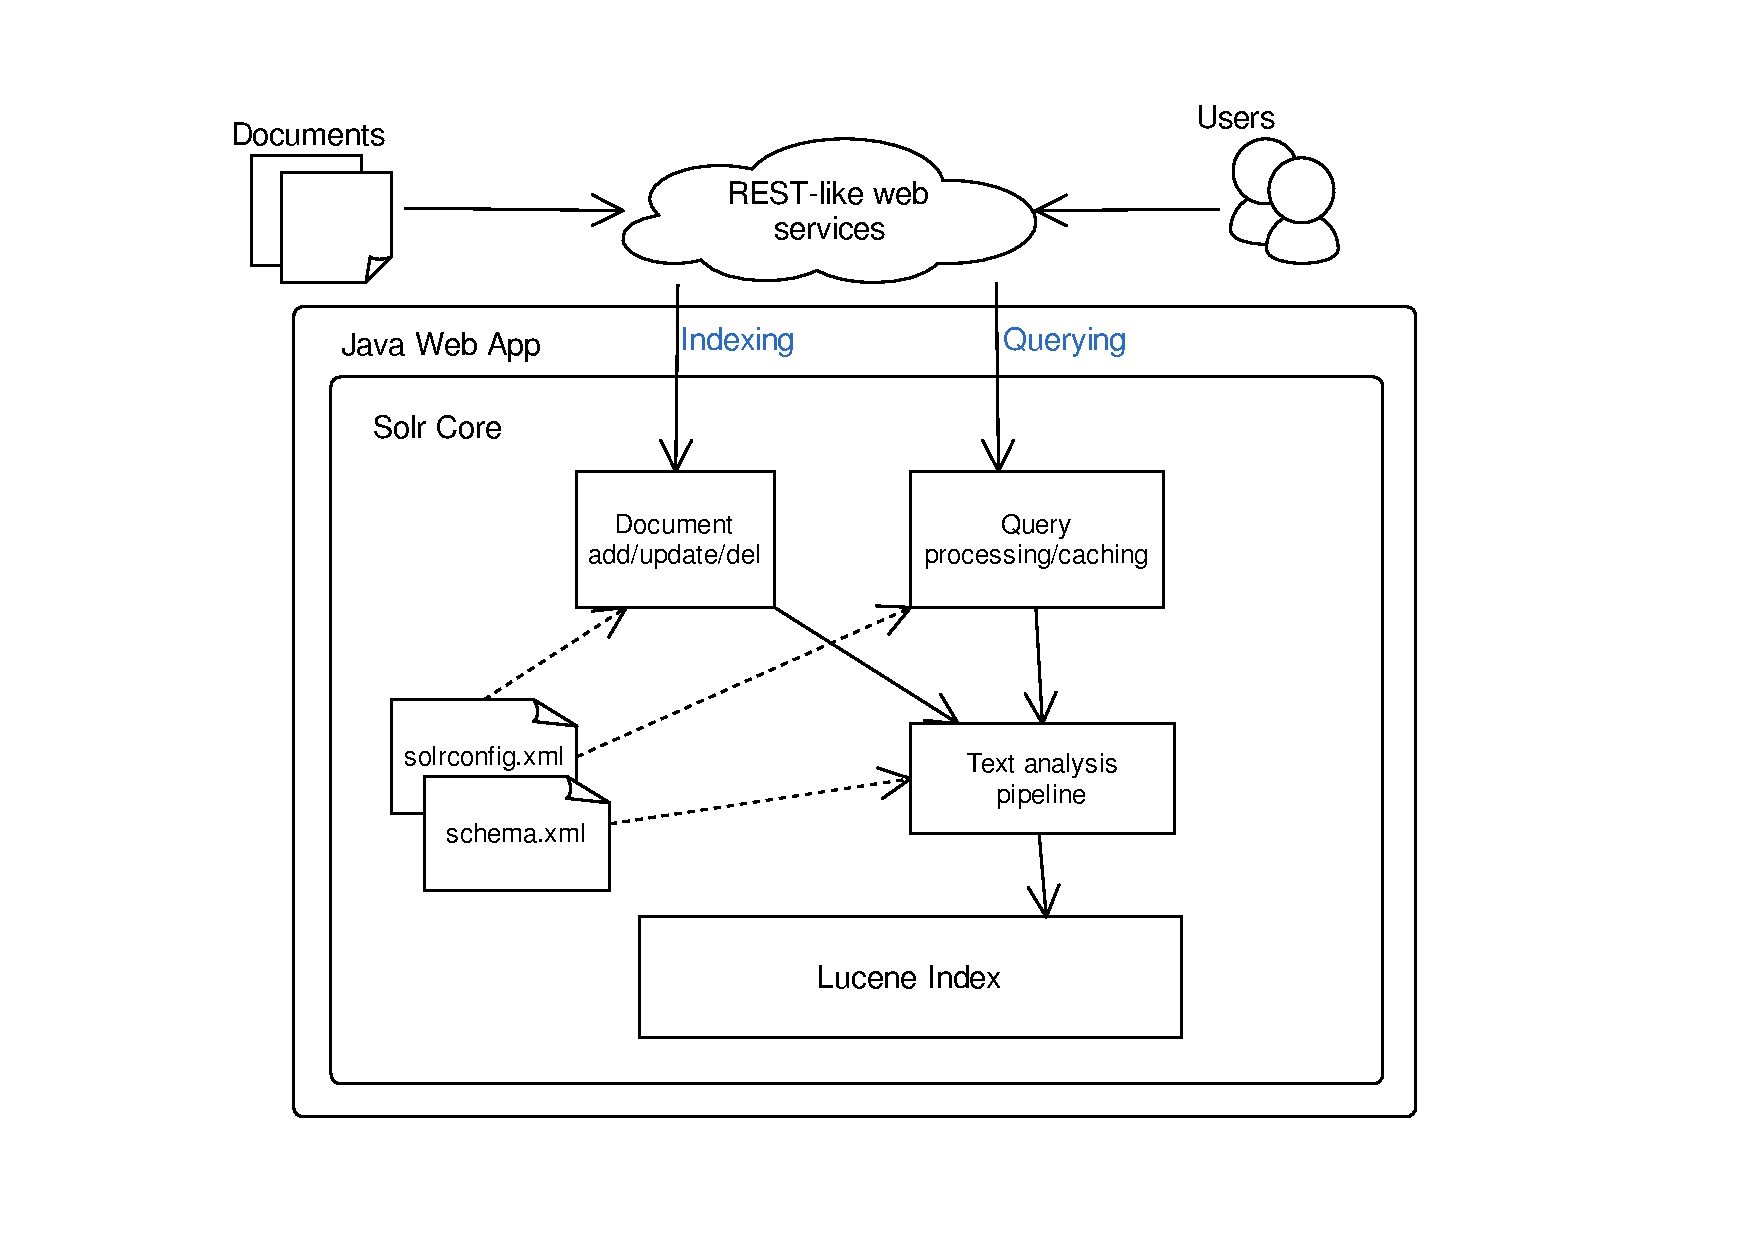
\includegraphics[scale=0.7]{solr}
    \caption{High level architecture of Solr system}
    \label{fig:solr}
  \end{figure} 

\subsection{Solr Configuration}
Solr installation requires JDK and any servlet container installed on a machine. Here configuration process for Apache Tomcat container is described.
We need to download Solr distribution that can be found on official Solr home page \cite{solr}. Solr is distributed as an archive. After unzipping the archive, the extracts have following directories:

\begin{itemize}
	\item \textbf{contrib/} - directory containing additional libraries to Solr, such as Data Import Handler, MapReduce, Apache UIMA, Velocity Template, and so on.
	\item \textbf{dist/} - directory providing distributions of Solr and other useful libraries such as SolrJ, UIMA, MapReduce, and so on.
	\item \textbf{docs/} - directory with documentation for Solr.
	\item \textbf{example/} - Jetty based web application that can be used directly.
	\item \textbf{Licenses/} - directory containing all the licenses of the underlying libraries used by Solr.
\end{itemize}

Copy the dist/solr.war file from the unzipped folder to \$CATALINA\_HOME/webapps/solr.war. Then point out to Solr location of home directory describing a collection. By collection in Apache Solr one imply a collection of Solr documents that represent one complete index. It's possible to choose one of the options:
\begin{itemize}
	\item \textbf{Java options} one can use following command so that the container picks up Solr collection information from the appropriate location:
	\begin{lstlisting}[language=bash]
$export JAVA_OPTS="$JAVA_OPTS -Dsolr.solr.home=/opt/solr/example"
	\end{lstlisting}
	\item \textbf{JNDI lookup} Or it is possible to configure the JNDI lookup for the java:comp/env/solr/home resource by pointing it to the Solr home directory. This can be done by creating a context XML file with some name (context.xml) in \$CATALINA\_HOME/conf/Catalina/localhost/context.xml and adding the following entries:
	\begin{lstlisting}[language=XML]
<?xml version="1.0" encoding="utf-8"?>
<Context docBase="<solr-home>/example/solr/solr.war" debug="0" crossContext="true">
<Environment name="solr/home" type="java.lang.String" value="<solr-home>/example/solr" override="true"/>
</Context>
	\end{lstlisting}
\end{itemize}

The Solr home directory contains configuration files and index-related data. It should consist of three directories:
\begin{itemize}
\item \textbf{conf/} - directory containing configuration files, such as solrconfig.xml and schema.xml
\item \textbf{data/} - default location for storing data related to index generated by Solr
\item \textbf{lib/} - optional directory for additional libraries, used by Solr to resolve any plugins
\end{itemize}

Configuring Solr instance requires defining a Solr schema and configuring Solr parameters.
\paragraph{Defining Solr schema}
Solr schema is defined in schema.xml file placed to conf/ directory of Solr home directory. Solr distribution comes with a sample schema file that can be changed for the needs of the project. Schema file defines the structure of the index, including fields and field types. The basic overall structure of schema file is following:
\begin{lstlisting}[language=XML]
	<schema>
	  <types>
	  <fields>
	  <uniqueKey>
	  <copyField>
	</schema>
\end{lstlisting}

The basic unit of data in Solr is document. Each document in Solr consist of fields that described in schema.xml file. By describing data in schema.xml Solr understand the structure of the data and what actions should be performed to handle this data. Here is an example of a field in schema file:
\begin{lstlisting}[language=XML]
	<field name="id" type="integer" indexed="true" stored="true" required="true"/>
\end{lstlisting}
Table \ref{tab:field.attrs} lists and explains major attributes of field element. 

\begin{table}[ht]
\begin{center}
\begin{tabular}{ | l | p{10cm}  | } 
 \hline
 Name & Description \\  \hline
 Default & default value if it is not read while importing a document \\ \hline
 Indexed & true if field should be indexed \\ \hline
 Stored & when true a field is stored in index store and is accessible while displaying results \\ \hline
 compressed & when true a field will be zipped, applicable for text-type fields \\ \hline
 multiValued & if true, field can contain multiple values in the same document. \\ 
 \hline
\end{tabular}
\caption{Major attributes of field element in schema.xml}
\label{tab:field.attrs}
\end{center}
\end{table}

Here is a fragment of schema file defining fields of a document in Citation Search Engine collection:
\begin{lstlisting}[language=XML]
    <fields>
     <field name="_version_" type="long" indexed="true" stored="true" multiValued="false"/>
     <field name="id" type="string" multiValued="false"/>
     <field name="text" type="text_en" indexed="true" multiValued="false"/>
     <field name="context" type="string" indexed="false" multiValued="false"/>
     <field name="path" type="string" indexed="false" multiValued="false"/>
     <field name="reference" type="string" indexed="false" stored="true" multiValued="true" />
    </fields>
\end{lstlisting}

Every document represent a citation with matching bibliographic references. In schema file we indicate that we want to index text field which is citation text. We store id of a citation, that is a generated value, calculated from the hash of the citation string. Specifying id is particularly useful for updating documents. We also store a context of a citation and path to the scientific article where citation was found. As citation can refer to multiple sources, we make reference field multivalued. 

In schema configuration file one can define field type, for example, string, date or integer and map them to Java class. This can be handy to define custom type. A field type includes following information:

\begin{itemize}
\item Name
\item Implementation class name
\item If field type is TextField, it will include a description of field analysis
\item Field attributes 
\end{itemize}

A sample field type description:
\begin{lstlisting}[language=XML]
	<fieldType name="text_ws" class="solr.TextField" positionIncrementGap="100">
  		<analyzer>
  		<tokenizer class="solr.WhitespaceTokenizerFactory"/>
  		</analyzer>
	</fieldType>
\end{lstlisting}

Other elements in the Solr schema file listed in Table \ref{tab:fields.others}:

\begin{table}[ht]
\begin{center}
\begin{tabular}{ | l | p{10cm}  | } 
 \hline
 Name & Description \\  \hline
 UniqueKey & specifies which field in documents is a unique identifier of a document, should be used if you ever update a document in the index\\ \hline
 copyField & used to copy field's value from one field to another \\ \hline
\end{tabular}
\caption{Description of some elements in schema.xml}
\label{tab:fields.others}
\end{center}
\end{table}
Once the schema is configured next step is to configure instance itself.

\paragraph{Configuring Solr parameters}
To configure Solr instance itself we need to describe solrconfig.xml and solr.xml files.

\begin{description}
\item[solr.xml] The solr.xml configuration is located in solr home directory and used for configuration of logging and advanced options to run Solr in a cloud mode.
\item[solrconfig.xml] The solrconfig.xml configuration file primarily provides you with an access to index-management settings, RequestHandlers, listeners, and request dispatchers. The file has a number of complex sections and mainly is changed when a specific need encounter. 
\end{description} 


 %\cite{solr.config}

\subsection{Enhanced search features}
Solr provides a number of additional features that can enhance search system. One of the feature we use is synonyms. To use this feature you need to specify synonyms.txt file with listed synonyms. This file is used by synonym filter to replace words with their synonyms. For example, a search for "DVD"may expand to "DVD", "DVDs", "Digital Versatile Disk" depending on the mapping in this file. This file can be also used for spelling corrections. Here is an example of synonyms.txt file:
\begin{lstlisting}
GB, gib, gigabyte, gigabytes
MB, mib, megabyte, megabytes
Television, Televisions, TV, TVs
Incident_error, error
\end{lstlisting}

Additionally, there are other configuration files that appear in the configuration directory. We are listing them in Table \ref{tab:solr.config} with the description of each configuration:
\begin{table}[ht]
\begin{center}
\begin{tabular}{ | l | p{10cm}  | } 
 \hline
 Name & Description \\  \hline
 protwords.txt & In this file, you can specify protected words that you do not wish to get stemmed. So, for example, a stemmer might stem the word "catfish" to "cat" or "fish".\\ \hline
 spellings.txt & In this file, you can provide spelling suggestions to the end user. \\ \hline
 elevate.txt & With this file, you can influence the search results and make your own results among the top-ranked results. This overrides Lucene's standard ranking scheme, taking into account elevations from this file. \\ \hline
 stopwords.txt & Stopwords are those that will not be indexed and used by Solr in the applications. This is particularly helpful when you really wish to get rid of certain words. For example, in the string, "Jamie and joseph," the word "and" can be marked as a stopword. \\ \hline
\end{tabular}
\caption{Additional configuration files in Solr}
\label{tab:solr.config}
\end{center}
\end{table}

\section{Meta Information storage}
\subsection{Configuration}
\section{Web search interface}
\subsection{Citation search page}
\subsection{Details page}

\chapter {Validation}
In which you show how well the solution works.

\chapter {Conclusion and Future Work}
In which we step back, have a critical look at the entire work, then conclude, and learn what lays beyond this thesis.

%%CS can be used as a search engine for the repository of scientific papers in research institutes, in universities, or in any
%%organization that deals with collection of scientific papers. /Users/aliya/Documents/Master Thesis/template/scgbib/LatexTemplates/msc-thesis/preamble.tex
%Parser enchancement
%meta information by advanced pdf-parsers
%personal storage
%distributed solution

%END Doc
%-------------------------------------------------------

\bibliographystyle{plain}
\bibliography{thesis}

\appendix
\chapter{User guide for Citation Search Engine deployment}
\section{Solr Installation}
\section{MongoDB Installation}
\section{Running parser}
\section{Search interface deployment}
\end{document}